\chapter{Data}

\section{Income Surveys}

\subsection{Survey of Income and Housing, 1981-2010}

The Survey of Income and Housing (SIH) is a hierarchical, clustered sample survey of income and expenditure patterns of the the Australian population, periodically conducted by the Australian Bureau of Statistics. It was first conducted in the 1981-2 fiscal year, followed by 1985-6, and then every two or three years from 1994-5. Microdata files were obtained as confidentialized unit record files (CURFs) for the surveys performed in 1981-2, 1985-6, 1994-5, 1995-6, 1996-7, 1997-8, 2000-1, 2002-3, 2005-6, 2007-8 and 2009-10.

Unlike the Census, which is a population survey, the SIH is conducted on just a sample of the population, and unit records are weighted by demographic variables in order to create a representative sample. Weights are produced at three levels of the survey hierarchy: household, income unit and person. (In addition, the SIH is occasionally produced simultaneously with the Housing Expenditure Survey, or HES, in which case further expenditure levels are recorded.) For the purposes of this project, only individual-level records are of interest, and so results are weighted by person weight, $PERS\_WT$.

\subsubsection{Survey Weights}

In all versions of the SIH, the $PERS\_WT$ variable for the $i$th record is computed as the reciprocal of that individual's probability of selection $\pi_i$:
$$ PERS\_WT_i = \frac{1}{\pi_i}, $$
$PERS\_WT_i$ can be interpreted as the number of individuals `represented' by record $i$. Note that the selection probabilities $\pi_i$, $i=1,\cdots,n$, need not sum to 1.

The survey data are weighted so as to be a representative sample of the Australian population. Weights are given in survey data as `person weights', an inverse selection probability for each individual in the population. 

\subsubsection{Occupational Coding}

A major drawback of using the SIH is that several different occupational codings are used, in different editions of the survey. 
\begin{enumerate}
\item 1981-82: occupations are coded using the three-digit 1976 Census coding standard (CCLO).
\item 1985-6, 1994-5: occupations are coded at the one-digit level using the ANSCO version 1 coding scheme.
\item 1995-6 to 1997-8: occupations are coded at the one-digit level using the ANSCO version 2 coding scheme.
\item 2007-8 and 2009-10: occupations are coded at the two-digit level using the ANZSCO conding scheme.
\end{enumerate}
To facilitate a comparison, civilian occupations are aligned to equivalent groups wherever possible. Military occupations are deemed non-comparable, and are discarded.

As described in the data appendix, to ensure comparability for skills, only individuals who report a full-time wage as their primary source of income are included. (** NB: later we might attempt \$ per hour)

\subsubsection{Educational Attainment}


\subsubsection{Income Coding}


\subsection{Census}

\section{Occupational Data}

One step which was skipped over in the informal analysis in the previous chapter was the assignment of occupations into task groups, on the basis of the occupational classification scheme. If task content is to be analyzed rigorously, and in greater detail than a simple three-occupation breakdown, a quantitative view of occupational task content is required. 

\subsection{Australia \& New Zealand Standard Classification for Occupations (ANZSCO)}

The standard classification scheme for occupations used in Australia, ANZSCO, simply lists by name the tasks a particular job title might be required to perform. These tasks are listed in an occupation-specific way, such that they cannot be compared between occupations. For example, under the unit group 2243: {\em Economists}, the required tasks include
\begin{quote}
{\em Analysing interrelationships between economic variables and studying the effects of government fiscal and monetary policies, expenditure, taxation and other budgetary policies on the economy and the community \citep[p.185]{Trewin2006}}
\end{quote}

{\em Statisticians} (unit group 2441) perform tasks that are largely similar to that of economists, even though the underlying theory that motivates their work may be somewhat different. A corresponding task entry for statisticians includes
\begin{quote}
{\em Defining, analysing and solving complex financial and business problems relating to areas such as insurance premiums, annuities, superannuation funds, pensions and dividends \citep[p.181]{Trewin2006}}
\end{quote}
Given the qualitative nature of this classification scheme, there is no obvious way to systematically formalise the similarity between economists and statisticians on the basis of the ANZSCO classification. However, alternative classification schemes do exist which include comparable task classifications.

\subsection{Occupational tasks: O*NET}\label{sec:onet}

The U.S. equivalent to the ANZSCO classification, the O*NET database, includes hundreds of quantitative scales for the level of work activities, knowledge types and abilities for individuals in each of approximately five hundred occupations. The data were constructed using expert surveys, and provide a very rich source of information about the activities that workers in each occupation actually undertake. For example, for the work activity {\em analyze data}, the occupations {\em economist} and {\em surgeon} score highly (6.58/7 and 5.49/7, respectively.) But for the work activity {\em Handle moving objects}, surgeons score 3.62/7, and economists score only 0.54/7.

We have mapped the ANZSCO (and its predecessors, various editions of ASCO and the CCLO) to the O*NET data, and sucessfully constructued a skill measure series for Australian occupational classification schemes. We then apply a transformation step, described by \citet{Firpo2011}, to build composite indexes for `automation,' `offshorability', and so on. These composite indexes provide a dependent variable which, along with levels of capital investment on an industry-by-industry basis, provide a basis by which changes in the occupational wage structure can be analyzed. The following five composite indexes are constructed for each occupation code:


\begin{enumerate}[A.]
\item Characteristics linked to Technological Change/Offshorability
\begin{enumerate}[1.]
\item Information Content 
  \begin{itemize}
  \item 4.A.1.a.1 Getting Information (JK)
  \item 4.A.2.a.2 Processing Information (JK) 
  \item 4.A.2.a.4 Analyzing Data or Information (JK) 
  \item 4.A.3.b.1 Interacting With Computers (JK) 
  \item 4.A.3.b.6 Documenting/Recording Information (JK)
  \end{itemize}
\item Automation/Routinization 
  \begin{itemize}
  \item 4.C.3.b.2 Degree of Automation 
  \item 4.C.3.b.7 Importance of Repeating Same Tasks 
  \item 4.C.3.b.8 Structured versus Unstructured Work (reverse) 
  \item 4.C.3.d.3 Pace Determined by Speed of Equipment 
  \item 4.C.2.d.1.i Spend Time Making Repetitive Motions
  \end{itemize}
\end{enumerate}
\item Characteristics linked to Non-Offshorability 
\begin{enumerate}[1.]
\item Face-to-Face
\begin{itemize}
  \item 4.C.1.a.2.l Face-to-Face Discussions 
  \item 4.A.4.a.4 Establishing and Maintaining Interpersonal Relationships (JK,B)
  \item 4.A.4.a.5 Assisting and Caring for Others (JK,B) 
  \item 4.A.4.a.8 Performing for or Working Directly with the Public (JK,B) 
  \item 4.A.4.b.5 Coaching and Developing Others (B)
\end{itemize}
\item On-Site Job 
\begin{itemize}
  \item 4.A.1.b.2 Inspecting Equipment, Structures, or Material (JK) 
  \item 4.A.3.a.2 Handling and Moving Objects 
  \item 4.A.3.a.3 Controlling Machines and Processes 
  \item 4.A.3.a.4 Operating Vehicles, Mechanized Devices, or Equipment 
  \item 4.A.3.b.4 Repairing and Maintaining Mechanical Equipment (*0.5) 
  \item 4.A.3.b.5 Repairing and Maintaining Electronic Equipment (*0.5)
\end{itemize}
\item Decision-Making 
\begin{itemize}
\item 4.A.2.b.1 Making Decisions and Solving Problems (JK) 
\item 4.A.2.b.2 Thinking Creatively (JK) 
\item 4.A.2.b.4 Developing Objectives and Strategies 
\item 4.C.1.c.2 Responsibility for Outcomes and Results 
\item 4.C.3.a.2.b Frequency of Decision Making
\end{itemize}
\end{enumerate}
\end{enumerate}

\begin{figure}
  \centering
  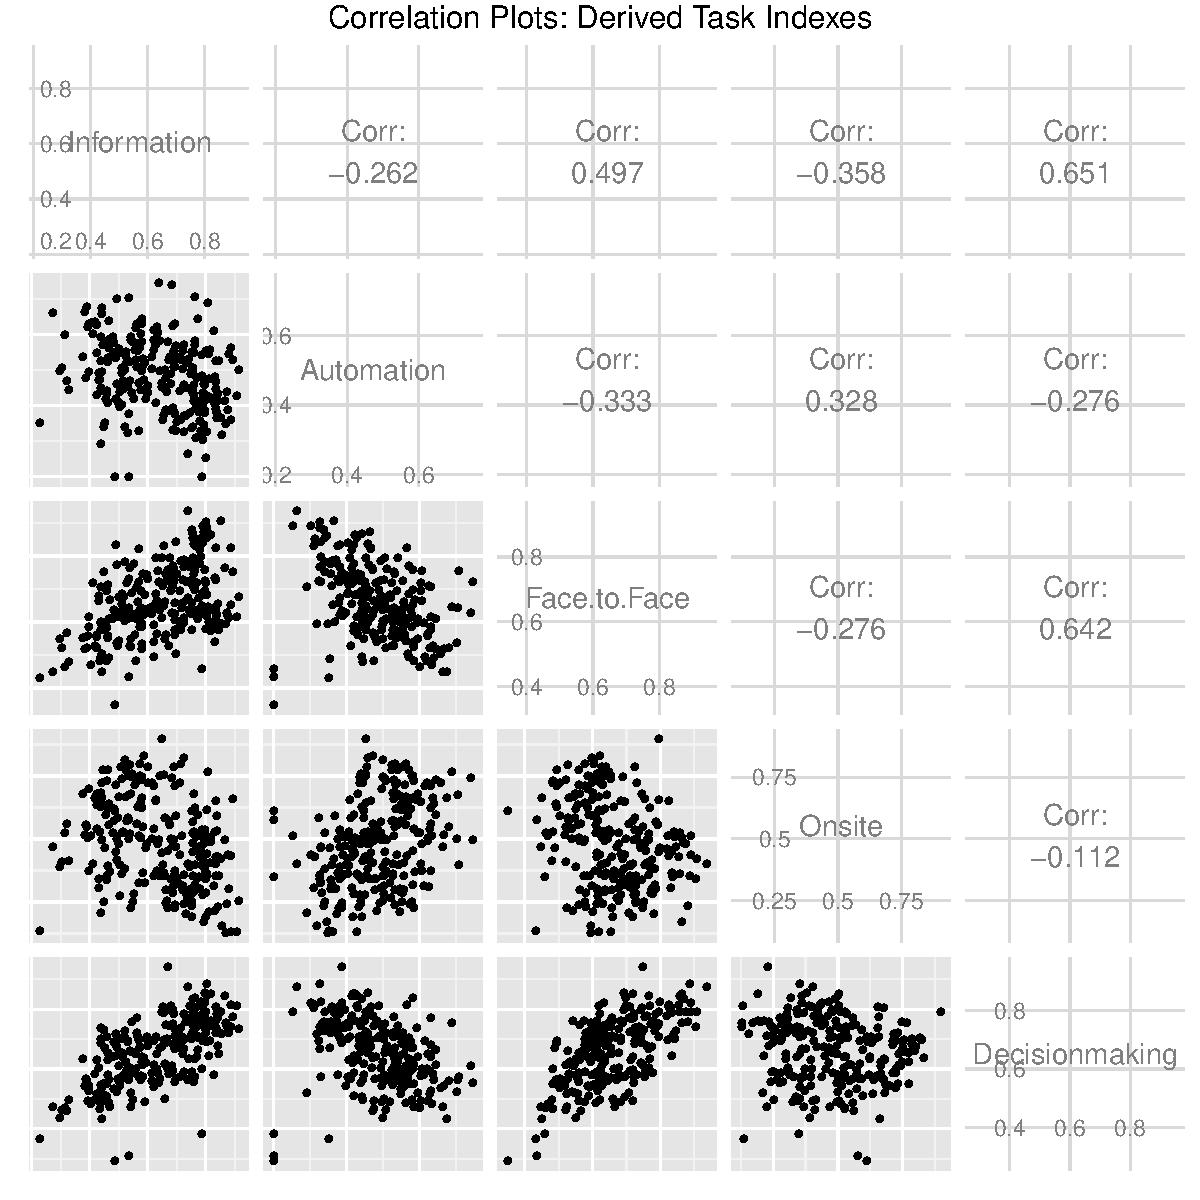
\includegraphics[width=\textwidth]{../figure/correl.pdf}
  \caption{Correlation plots: occupational task indexes for jobs at the ANZSIC 3-digit level.}
  \label{fig:correl}
\end{figure}

The correlation between each job index is plotted in Figure~\ref{fig:correl}. Notice that the job indexes are not perfectly mutually independent. As might be expected, `information content' is positively correlated with `face-to-face' roles ($\rho=0.497$) and decision-making ($\rho=0.651$), but negatively correlated with the job requiring on-site presence ($\rho=-0.358$). `Routinization' is negatively correlated with both face-to-face contact ($\rho=-0.33$) and decision-making ($\rho=-0.276$).

%%% Local Variables: 
%%% mode: latex
%%% TeX-master: "paper"
%%% End: 
